\documentclass{article}

\usepackage{fancyhdr}
\usepackage{extramarks}
\usepackage{amsmath}
\usepackage{amsthm}
\usepackage{amsfonts}
\usepackage{tikz}
\usepackage[plain]{algorithm}
\usepackage{algpseudocode}
\usepackage{graphicx}
\usepackage{gensymb}
\usepackage{hyperref}
\usepackage{enumitem}

\DeclareRobustCommand{\bbone}{\text{\usefont{U}{bbold}{m}{n}1}}

\DeclareMathOperator{\EX}{\mathbb{E}}% expected value

\graphicspath{{./images/}}

\usetikzlibrary{automata,positioning}

%
% Basic Document Settings
%

\topmargin=-0.45in
\evensidemargin=0in
\oddsidemargin=0in
\textwidth=6.5in
\textheight=9.0in
\headsep=0.25in

\linespread{1.1}

\pagestyle{fancy}
\lhead{\hmwkAuthorName}
\chead{\hmwkClassShort\ \hmwkTitle}
\rhead{\firstxmark}
\lfoot{\lastxmark}
\cfoot{\thepage}

\renewcommand\headrulewidth{0.4pt}
\renewcommand\footrulewidth{0.4pt}

\setlength\parindent{0pt}

%
% Create Problem Sections
%

\newcommand{\enterProblemHeader}[1]{
    \nobreak\extramarks{}{Problem {#1} continued on next page\ldots}\nobreak{}
    \nobreak\extramarks{{#1} (continued)}{{#1} continued on next page\ldots}\nobreak{}
}

\newcommand{\exitProblemHeader}[1]{
    \nobreak\extramarks{{#1} (continued)}{{#1} continued on next page\ldots}\nobreak{}
    % \stepcounter{#1}
    \nobreak\extramarks{{#1}}{}\nobreak{}
}

\setcounter{secnumdepth}{0}
\newcounter{partCounter}

\newcommand{\problemNumber}{0.0}

\newenvironment{homeworkProblem}[1][-1]{
    \renewcommand{\problemNumber}{{#1}}
    \section{\problemNumber}
    \setcounter{partCounter}{1}
    \enterProblemHeader{\problemNumber}
}{
    \exitProblemHeader{\problemNumber}
}

%
% Homework Details
%   - Title
%   - Class
%   - Author
%

\newcommand{\hmwkTitle}{DRL Assignment}
\newcommand{\hmwkClassShort}{RBE 595}
\newcommand{\hmwkClass}{RBE 595 --- Reinforcement Learning}
\newcommand{\hmwkAuthorName}{\textbf{Arjan Gupta}}

%
% Title Page
%

\title{
    \vspace{2in}
    \textmd{\textbf{\hmwkClass}}\\
    % \textmd{\textbf{\hmwkTitle}}\\
    \textmd{\textbf{Deep Reinforcement Learning Assignment}}\\
    \vspace{3in}
}

\author{\hmwkAuthorName}
\date{}

\renewcommand{\part}[1]{\textbf{\large Part \Alph{partCounter}}\stepcounter{partCounter}\\}

%
% Various Helper Commands
%

% Useful for algorithms
\newcommand{\alg}[1]{\textsc{\bfseries \footnotesize #1}}

% For derivatives
\newcommand{\deriv}[2]{\frac{\mathrm{d}}{\mathrm{d}#2} \left(#1\right)}

% For compact derivatives
\newcommand{\derivcomp}[2]{\frac{\mathrm{d}#1}{\mathrm{d}#2}}

% For partial derivatives
\newcommand{\pderiv}[2]{\frac{\partial}{\partial #2} \left(#1\right)}

% For compact partial derivatives
\newcommand{\pderivcomp}[2]{\frac{\partial #1}{\partial #2}}

% Integral dx
\newcommand{\dx}{\mathrm{d}x}

% Alias for the Solution section header
\newcommand{\solution}{\textbf{\large Solution}}

% Probability commands: Expectation, Variance, Covariance, Bias
\newcommand{\E}{\mathrm{E}}
\newcommand{\Var}{\mathrm{Var}}
\newcommand{\Cov}{\mathrm{Cov}}
\newcommand{\Bias}{\mathrm{Bias}}

\begin{document}

\maketitle

\nobreak\extramarks{Problem 1}{}\nobreak{}

\pagebreak

\begin{homeworkProblem}[Problem 1]
    What are the two sources of error in Deep RL with function approximation?

    \subsection{Answer}

    The two sources of error in Deep RL with function approximation are as follows:

    \begin{itemize}
        \item \textbf{Bootstrapping error} --- This is the error that arises due to the use of
        bootstrapping. Bootstrapping is the process of using the value of a successor state to
        update the value of a state. This is done in TD methods. The error is the difference
        between the target value and the current estimate value.
        \item \textbf{Approximation error} --- This is the error defined as the difference
        between the true value function and the approximate value function. This error arises
        due to the use of function approximation itself.
    \end{itemize}

\end{homeworkProblem}

\nobreak\extramarks{Problem 2}{}\nobreak{}

\pagebreak

\begin{homeworkProblem}[Problem 2]
    In TD learning with a neural network what are we trying to minimize? What are we trying to
    maximize?

    \subsection{Answer}

    In general with any deep TD learning method, we aim to minimize the error between the target value
    and the current estimate Q-value. We try to maximize the value of the current state by choosing
    the action that maximizes the value of the next state.\\

    We can use the example of gradient Q-learning to answer this question more specifically.
    In gradient Q-learning, we are trying to minimize the error given by the loss function as follows:

    \begin{align*}
        e(w) &= \frac{1}{2} \left[ Q_w(s, a) - \left( r + \gamma \max_{a'} Q_{w'}(s', a') \right) \right]^2\\
    \end{align*}

    We are trying to maximize the value of the current state by choosing the action that maximizes
    the value of the next state. This is done by updating the weights of the neural network.

\end{homeworkProblem}

\nobreak\extramarks{Problem 2}{}\nobreak{}

\pagebreak

\nobreak\extramarks{Problem 3}{}\nobreak{}

\begin{homeworkProblem}[Problem 3]
    What is the main benefit of deep neural networks in function approximation compared to linear
    method? What is the linear function approximation useful for?

    \subsection{Answer}

    Deep neural networks (DNNs) have helped reinforcement learning become more powerful and practical.
    DNNs can be used to approximate the value function as a non-linear function of the state. This
    is more powerful than linear function approximation, which can only approximate the value function
    as a linear function of the state. A general advantage of DNNs is also that they learn their own
    features, which is not the case with linear function approximation.\\

    Linear function approximation are still useful, however. Their advantage is that they can
    be used to verify theoretical results (in academia, for example). The mathematical analysis
    of linear function approximation is much easier than that of non-linear function approximation,
    which is why linear function approximation is still useful.
\end{homeworkProblem}

\pagebreak

\nobreak\extramarks{Problem 4}{}\nobreak{}

\begin{homeworkProblem}[Problem 4]
    In DQN, what is the purpose of the target network and value network?

    \subsection{Answer}

    In DQN, two separate neural networks are used: the target network and the value network. The
    target network is used to estimate the target value, whereas the value network is used to estimate
    the Q-value. The purpose of having two separate networks is to serve as one of the two features
    of DQN that mitigates the problem of divergence (or weaker convergence) that occurs in
    gradient Q-learning. The other feature is experience replay.\\
    
    We can provide more context on how DQN achieves this mitigation, as follows.
    The target network is updated less frequently than the value network for each mini-batch of
    $(s, a, r, s')$ tuples from the experience replay buffer. This is done to make the target
    network more stable. The target network is updated as follows:

    \begin{align*}
        w_{i+1} &= w_i + \alpha \left[ Q_w(s, a) - r - \gamma \max_{a'} Q_{\overline{w}}(s', a') \right] \frac{\partial Q_{{w}}(s, a)}{\partial w}
    \end{align*}

    Where the first Q in the square brackets is the value network, and the second Q is the target
    network. The second Q remains `fixed' for a certain number of iterations. This is akin to
    the optimal value function being fixed while the value function for all the other states is
    being updated. 

\end{homeworkProblem}

\pagebreak

\nobreak\extramarks{Problem 5}{}\nobreak{}

\begin{homeworkProblem}[Problem 5]
    In the Deep Q-learning method, which are true:

    \begin{enumerate}[label=(\alph*)]
        \item epsilon-greedy is required to ensure exploration.
        \item exploration is taken care of by the randomization provided by experience replay.
    \end{enumerate}

    \subsection{Answer}
    
    (a) is true. Epsilon-greedy is required to ensure exploration as seen in the
    `Deep Q-learning with Experience Replay' paper's algorithm. This is because the action
    selection policy is greedy. This means that the agent will always choose the action that
    maximizes the Q-value. So, in order to ensure exploration, epsilon-greedy action selection
    is used.\\

    (b) is false. Exploration is not taken care of by the randomization provided by experience replay.
    Experience replay is used to break the correlation between consecutive samples. This is done by
    storing the samples in a buffer and sampling from the buffer randomly. This is done to make the
    training process more stable. However, this does not take care of exploration because the agent
    is not experiencing or simulating any new orders of states. The agent is only experiencing the
    same states in a different order.
\end{homeworkProblem}

\pagebreak

\nobreak\extramarks{Problem 6}{}\nobreak{}

\begin{homeworkProblem}[Problem 6]

    Does Q-learning learn the outcome of exploratory actions? (Refer to the Cliff walking example).

    \subsection{Answer}

    Yes, Q-learning learns the outcome of exploratory actions. This is because Q-learning is an
    off-policy TD control algorithm. In the context of the Cliff walking example, this means that
    Q-learning learns the optimal action-value function, $q_*$, which is closest to the cliff. 
    The behavior policy takes exploratory actions, and the target policy is greedy. This
    causes makes it so that initially, the agent falls off the cliff a lot, but eventually, the agent
    learns to avoid the cliff and converges to the optimal action-value function, $q_*$. This is why the
    graph of the sum of rewards per episode for Q-learning is initially very low, but eventually
    converges to a high value. The graph is shown below:

    \begin{center}
        % 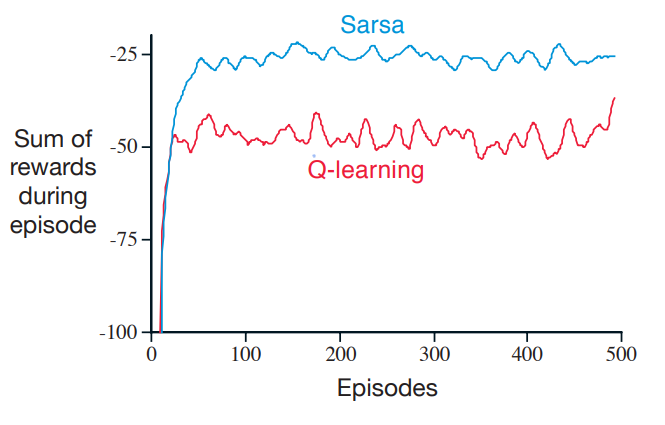
\includegraphics[scale=0.5]{q_learning_cliff_walking.png}
    \end{center}

\end{homeworkProblem}

\pagebreak

\nobreak\extramarks{Problem 7}{}\nobreak{}

\begin{homeworkProblem}[Problem 7]

    What is the advantage of Double Q-learning over Q-learning?

    \subsection{Answer}

    The advantage of Double Q-learning over Q-learning is that Double Q-learning is less prone to
    bias than Q-learning. Specifically, Q-learning is biased toward the maximum value action, which
    is also known as maximization bias. This is because Q-learning uses the maximum value action
    to update the value of a state.\\

    In contrast, Double Q-learning is not biased toward the maximum value action. This is because
    Double Q-learning uses two action-value functions, $Q_1$ and $Q_2$, to update the value of a state.
    With probability $0.5$, Double Q-learning uses either $Q_1$ or $Q_2$ to update the value of a state.
    Now, for example, the action is picked as per $Q_1$, then that action is probably not the maximum
    value action as per $Q_2$. This way, for a given state, we have two estimates of the value of the
    maximum value action. This reduces the bias of Double Q-learning and is hence the advantage over
    Q-learning.


\end{homeworkProblem}

\end{document}